\documentclass[11pt]{amsart}

% Standard letter size paper with 1inch margins
\usepackage[letterpaper, margin=1in]{geometry}
\usepackage{float}
% Useful packages 
\usepackage{amsmath, amssymb, amsthm, amsaddr}
\usepackage{enumerate, subcaption, graphicx, hyperref}


\title{AMATH 482/582: Homework 1}
\author{Sathvik Chinta} % first and last name

\date{\today} % you can also just type the date instead of "\today"

\begin{document}

\maketitle 

\begin{abstract}
    Using the Fast Fourier Transform algorithm alongside a Guassian Noise filter, we were able to succesfully
    de-noise acoustic data of a submarine located within Puget Sound and track its position over a 24 hour
    period of time. 
    % Your report should contain a brief, 100 word abstract describing what is contained in 
    % the document and what you did. {\bf Don't forget 6 pages max}.
\end{abstract}


\section{Introduction and Overview}\label{sec:Introduction}
Imagine we are given the following problem:
There is a submarine traveling thorugh Puget Sound. We've been tasked with finding the submarine
and tracking it over a 24 hour period. We've been given a 64 x 64 x 64 grid of acoustic data points at 
30 minute intervals, but the data is noisy. The submarine is also moving, so we need to determine 
its path if we want to find it. 

Since we're dealing with acoustic frequencies, we should immediately be thinking of Fourier Transforms.
These will be key in order for us to find the path of the submarine. 

% Here you will give a brief introduction to the problem you solved. Including 
% some discussion of relevant literature and background. 

% Make sure you use the correct citation commands (i.e., \texttt{$\backslash$cite}) to keys 
% from your bib file like this \cite{example-article-citation}. If you want 
% to cite more than one reference simply use \cite{example-article-citation, example-book-citation}. You can grab latex citations 
% from \href{https://scholar.google.com}{Google Scholar}. Just keep in mind that they often 
% need to be cleaned up.

\section{Theoretical Background}\label{sec:theory}
Imagine we have multiple frequencies being combined together into a single signal. Simply observing the shape of the 
signal would be very hard to interpret. However, we know that there are multiple underlying frequencies that have
been combined in order to give us the output signal. The Fourier Transform is an effective method to decompose 
such a signal into its underlying frequencies. In our case, since we are dealing with noisy acoustic data underwater, 
we can stand to believe that there will be multiple frequencies (corresponding to the noise and the submarine). If
we were to scrub away the noise, then the highest frequency would be the submarine.

We know the data is noisy. As such, we can use an interesting property of the Fourier Transform in order
to help get rid of the noise. Let the function be represented by the following: 

\[f(x) = g(x) + \xi\]

Where $\xi$ is the noise and $f(x)$ is the submarine data. The clean data should then be represented
by $g(x)$, so the question is how do we get rid of the noise. If we assume the noise is random 
in distribution with mean 0, then taking the Fourier Transform of the random variable will still be some random variable.
As such, we can write this as 

\[\hat{f(x)} = \hat{g(x)} + \xi\]

We have a distribution over time (one point at every 30 mintues for 24 hours). If we imagine that there are
$n$ number of such points, then if we were to take the average of this fourier transform over time, it
would become 

\[\frac{1}{n}\sum_{n=0}^{n-1}\hat{f(x)} = \frac{1}{n}\sum_{n=0}^{n-1}\hat{g(x)} + \frac{1}{n}\sum_{n=0}^{n-1}\xi\]

However, since $\xi$ is randomly distributed with mean 0, the noise should approach 0 as well. So,
this should simplify to 

\[\frac{1}{n}\sum_{n=0}^{n-1}\hat{f(x)} = \frac{1}{n}\sum_{n=0}^{n-1}\hat{g(x)}\]

Effectively meaning that we have dealt with the noise.
Once we have gotten rid of the noise, we should be able to scan through the fourier transform 
and find the highest frequency. Since there should be no other frequencies in the data, we can 
use this frequency to find the value of the central frequency (and it's $x, y, z$ coordinates). 

When we create a filter to denoise the data when finding the path, we can extend the Gaussian filter
to three dimensions. In two dimensions, the filter is 

\[G(x, y, \sigma) = e^{-\frac{x^2 + y^2}{2\sigma^2}}\]

Where $\sigma$ is chosen by us. We can extend this definition to three dimensions by just adding another
dimension $z$. In this case, the Gaussian Filter would become 

\[G(x, y, z, \sigma) = e^{-\frac{x^2 + y^2 + z^2}{2\sigma^2}}\]

We will use this filter to attempt to de-noise along the path that the submarine takes. We can also center 
this around the max frequency in order to better reduce noise around the sub. Let $(a, b, c)$
be the x, y, and z coordinates of the max frequency. Our Gaussian filter would then look like 

\[G(x, y, z, \sigma) = e^{-\frac{(x - a)^2 + (y - b)^2 + (z - c)^2}{2\sigma^2}}\]

Also, the transform would be given to us from range -32 to 32, but we want our range to be from 0 till 64.
So, we will add 32 to each dimension as well to get the final Gaussian filter as 

\[G(x, y, z, \sigma) = e^{-\frac{(x - a + 32)^2 + (y - b + 32)^2 + (z - c + 32)^2}{2\sigma^2}}\]

% You dedicate this section to the theoretical background of the methods and frameworks 
% that you used in your homework. This is not meant to reproduce material from the lectures
%  or references you used but rather to demonstrate your understanding of the 
%  mathematical foundations of the methods and algorithms. You can create equations like this 
%  \begin{equation*}
%      f(x) = \int_A \sin( \pi x) dx.
%  \end{equation*}
%  You do not need to label your equations unless they are referenced in the text. In that 
%  case simply use 
%  \begin{equation}\label{eq:meaningful-label}
%       - \frac{\partial^2 u}{\partial x^2} = \sin ( \pi x).
%  \end{equation}
% Also look up the \texttt{align} or \texttt{aligned} environments if you want multi-line 
% equations. You can then reference your equations in text using the $\backslash$\texttt{eqref}
% command as such \eqref{eq:meaningful-label}. 

\section{Algorithm Implementation and Development}\label{sec:algorithms}

For this assignment, I used Python. I used NumPy to do all mathematical operations and the Fourier Transforms. 
I used Matplotlib to plot the data and the path of the submarine, as well as any other plots. 

Within numpy, I used the following functions:
\subitem \texttt{np.reshape()} to reshape the data into a 3D array.
\subitem \texttt{np.fft.fftshift()} to shift the fourier transform data. 
\subitem \texttt{np.fft.fftn()} to take the fourier transform of the data in $n$ dimensions (3 in our case).
\subitem \texttt{np.size()} to find the size of the data.
\subitem \texttt{np.argmax()} to find the index of the max value in the fourier transform (used to find the central frequency).
\subitem \texttt{np.abs()} to find the absolute value of the fourier transform.
\subitem \texttt{np.real()} to find the real part of the fourier transform.
\subitem \texttt{np.unravelIndex()} to convert the flat index of the central frequency to a tuple of indices,
which was then fed into the Gaussian function 
\subitem \texttt{np.exp()} to take the exponential of the Gaussian function.
\subitem \texttt{np.fft.ifftn()} to take the inverse fourier transform after applying the Gaussian function.
\subitem \texttt{np.fft.ifftshift()} to shift the inverse fourier transform data.

Within matplotlib, I used the following functions:
\subitem \texttt{plt.plot()} to plot the data in two dimensions.
\subitem \texttt{plt.axes(projection = '3d')} to plot the data in three dimensions.

% Here you discuss the algorithms and software packages that you used. Not much to it. 
% Just make sure you cite the packages properly and avoid including code. 
% You are welcome to use \LaTeX packages that are specifically designed to show 
% algorithms such \href{https://www.overleaf.com/learn/latex/Algorithms}{as this}, but it is 
% not always worth the effort and real estate. 


\section{Computational Results}\label{sec:results}

Averaging over time after taking the FFT in order to reduce noise, I go the highest frequency as 90. Looking for the $x, y, z$ coordinates
of the max frequency, I found the central frequency as (39, 49, 10) with value 90. 

Through my testing, I found the ideal value of $\sigma$ to be used in my Gaussian filter to be 15. 

After computing the Gaussian filter and using the central frequency coordinates within them, I multiplied 
my filter by the result of the Fourier Transform. I then took the inverse Fourier Transform, and repeated the
process for each data point (every 30 minutes for the entire 24 hour timespan). This resulted in 
the following path for the x-y plane:
\begin{figure}[H]
    \centering
    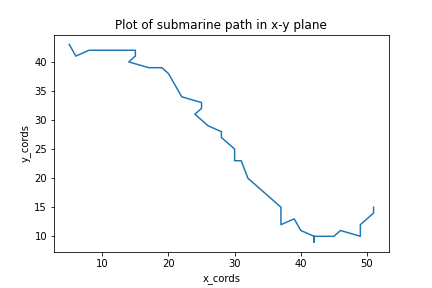
\includegraphics[width=0.4\textwidth]{./images/submarine_path_xy.png}
    \caption{A plot of the x-coordinates and the y-coordinates of the submarine path over the 
    entire 24 hours\\\\\\}
    \label{fig:subXY}
\end{figure}
We can now clearly see the path that the submarine is taking. The original data itself is in 3 dimensions, 
so while we can't paint the whole picture just yet (we will graph in 3 dimensions later on), we can 
see the general shape of the path that the submarine is taking.

This is what the path looks like in 3 dimensions: 
\begin{figure}[H]
    \centering
    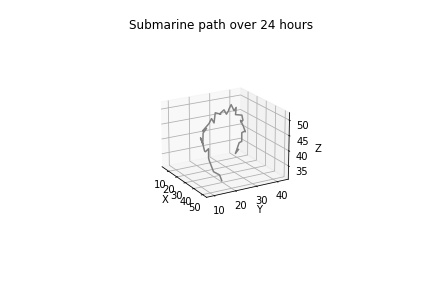
\includegraphics[width=0.5\textwidth]{./images/submarine_path_3d.png}
    \caption{A plot of the of the submarine path over the 
    entire 24 hours in all 3 dimensions}
    \label{fig:sub3D}
\end{figure}

We can see that the path is very clear, with minimal (if any) noise. The jagged lines might be 
a result of the noise, but doing a bit of research into the subject reveals that submarines do 
in fact take rapid turns in order to avoid detection. 

% This is perhaps the most important section of your report. You want to dedicate more space 
% here and present your numerical results in a clear, concise and meaningful way. Also 
% include a discussion of your numerics. Think hard about how you can use 
% your space most efficiently. For example, include subplots and multiple error curves on the 
% same plot etc. Ask us for advice when the time comes. 

% You will most definitely need tables and figures. So here is an example. 

% \begin{table}[htp]
%     \centering
%     \begin{tabular}{| l | c|c | r |}
%          \hline
%          row 1 & column 1  & column 2  \\ \hline
%          row 2 & column 1 & column 2 \\ 
%          row 3 & column 1 & column 2 \\ \hline
%     \end{tabular}
%     \caption{Don't forget to include a caption for your table. Say a few words about what is 
%     being shown.}
%     \label{tab:meaningful-label}
% \end{table}

% Make sure your table is labeled and referenced withing the text using $\backslash$\texttt{ref} as such Table~\ref{tab:meaningful-label}. In fact, you can 
% use $\backslash$\texttt{ref} to cite anything else in the document such as 
% sections (ex. Section~\ref{sec:Introduction}). This will create hyperlinks in your 
% pdf after compilation and automatically update the numbers and tags whenever you change 
% anything. 

% Figures are very similar to tables. Here's an example: 

% % \begin{figure}[htp]
% %     \centering
% %     \includegraphics[width=0.4\textwidth]{./Figs/fig1.pdf}
% %     \caption{Include a descriptive caption for your figure. Also make sure all 
% %     legends, axis labels, and titles are large enough to be readable. You might have 
% %     to reproduce the plots from Python or MATLAB with larger fonts for this purpose. It 
% %     can be annoying the first time you do it but it is crucial.}
% %     \label{fig:meaningful-label}
% % \end{figure}

% You may also need to include multiple figures: 

% % \begin{figure}
% %     \centering
% %     \begin{subfigure}[b]{.3\textwidth}
% %     \includegraphics[width=\textwidth]{./Figs/fig1.pdf}
% %     \caption{First subfigure}
% %     \label{subfig:first}
% %     \end{subfigure}
% %     \begin{subfigure}[b]{.3\textwidth}
% %     \includegraphics[width=\textwidth]{./Figs/fig2.pdf}
% %     \caption{First subfigure}
% %     \label{subfig:second}
% %     \end{subfigure}
% %     \begin{subfigure}[b]{.3\textwidth}
% %     \includegraphics[width=\textwidth]{./Figs/fig3.pdf}
% %     \caption{First subfigure}
% %     \label{subfig:third}
% %     \end{subfigure}
% %     \caption{Caption for entire figure. You don't need to use captions for subfigs so 
% %     feel free to eliminate the subcaption texts to just have the A, B, C labels.}
% %     \label{fig:meaningful-label-2}
% % \end{figure}

% Once again, make sure all your figures are referenced like Figure~\ref{fig:meaningful-label}
% or Figure~\ref{subfig:first} in the text body of the report and discussed 
% in detail. This is where you will make observations about your results and we will 
% look at these very closely. 

% Also note, I am using PDF figures. These give you the best looking graphs but PNG works 
% well too. I advise staying away from JPG as it always looks weird and low quality.]
% Both Python and MATLAB can output figures in PDF or PNG.

\section{Summary and Conclusions}\label{sec:conclusions}

Even with very messy data in a higher dimension space, Fourier Transforms are still very effective at finding 
the most significant features. Guassian noise filters are also very effective, and applicable to a wide variety 
of use cases. We were succesfully able to find the path of the submarine inside of Puget Sound over the 24 hour
time period. 
% Wrap up your report with a brief summary of what you did and what you discovered. 
% Finish with some conclusions and possibly future directions if any. 

\section*{Acknowledgements}

I am thankful to Professor Hosseini for introducing us to the concept of Fourier Transforms and explaining
their significance. I am also grateful to the YouTube Channel "3Blue1Brown" by Grant Sanderson for providing
a visual explanation for the intuition behind Fourier Transforms/series, and how they can be used to find 
signals within data. 

I am very thankful to my peers taking the class alongside me, they have helped me understand the material as well
as provide a reference to compare my results against. I interacted with them both through Canvas discussion boards
as well as Discord chat. 
% Make sure you you clearly state any help you received including collaborations 
% with your peers. Help from TAs or other mentors, professors, etc that helped you 
% with your assignment. Here's a formal example: 

% The author is thankful to Prof. X for useful discussions about the QR algorithm. 
% We are also thankful to Dr. Strange for suggesting the JAX software package for 
% automatic differentiation. Furthermore, our peer Jean Grey was helpful in 
% implementation of spectral clustering in Python.

\bibliographystyle{abbrv}
\bibliography{HW_References} % make sure this matches the .bib file for your corresponding document. You also have to maintain your references in the .bib file 
\cite{Hunter:2007}
\cite{harris2020array}
\cite{hosseini3_2022}
\cite{hosseini7_2022}
\end{document}
